%%%%%%%%%%%%%%%%%%%%%%%%%%%%%%%%%%%%%%%%%
% APA Assignment Article
% LaTeX Template
% Version 2.0 (February 7, 2023)
%
% This template originates from:
% https://www.LaTeXTemplates.com
%
% Author:
% Vel (vel@latextemplates.com)
%
% License:
% CC BY-NC-SA 4.0 (https://creativecommons.org/licenses/by-nc-sa/4.0/)
%
% NOTE: The bibliography needs to be compiled using the biber engine.
%
%%%%%%%%%%%%%%%%%%%%%%%%%%%%%%%%%%%%%%%%%

%----------------------------------------------------------------------------------------
%	PACKAGES AND OTHER DOCUMENT CONFIGURATIONS
%----------------------------------------------------------------------------------------

\documentclass[
	letterpaper, % Paper size, use either a4paper or letterpaper
	10pt, % Default font size, can also use 11pt or 12pt, although this is not recommended
	unnumberedsections, % Comment to enable section numbering
	twoside, % Two side traditional mode where headers and footers change between odd and even pages, comment this option to make them fixed
]{APAAssignment}

\addbibresource{bibliography.bib} % BibLaTeX bibliography file

\runninghead{MICS CYBER 252, Fall-2024 Hands On Lab Unit 10} % A shortened article title to appear in the running head, leave this command empty for no running head

\footertext{\textit{Hands On Lab 10} (MICS CYBER 252, Fall -2024)} % Text to appear in the footer, leave this command empty for no footer text

\setcounter{page}{1} % The page number of the first page, set this to a higher number if the article is to be part of an issue or larger work

%----------------------------------------------------------------------------------------
%	TITLE SECTION
%----------------------------------------------------------------------------------------

\usepackage[title,toc,titletoc]{appendix}
\usepackage{titlesec}
\usepackage{lscape}
\usepackage{fontawesome}

\title{Hands On Lab: Unit 10 \\ MICS-252, Fall 2024 \\ Incident Response Linux} % Article title, use manual lines breaks (\\) to beautify the layout

% Authors are listed in a comma-separated list with superscript numbers indicating affiliations
% \thanks{} is used for any text that should be placed in a footnote on the first page, such as the corresponding author's email, journal acceptance dates, a copyright/license notice, keywords, etc
% Affiliations are output in the \date{} command
\date{UC Berkeley School of Information \\
MICS Course 252 Fall 2024 (Kristy Westphal)
}


\author{
	Prepared by: Karl-Johan Westhoff \\
	email: \href{mailto:kjwesthoff@berkeley.edu}{kjwesthoff@berkeley.edu}
}


% % Full-width abstract
% \renewcommand{\maketitlehookd}{%
% 	\begin{abstract}
% 		\noindent Lorem ipsum dolor sit amet,rta porttitor.
% 	\end{abstract}
% }

%----------------------------------------------------------------------------------------

\setcounter{tocdepth}{5}
\setcounter{secnumdepth}{5}
\usepackage[title]{appendix}

\begin{document}
\onecolumn
\maketitle % Output the title section

%----------------------------------------------------------------------------------------
%	ARTICLE CONTENTS
%----------------------------------------------------------------------------------------


\section{Introduction}
We are given a snapshot of some files from a Linux host which has been compromised.


\section{Process}


\subsection{Open source information}
Linux version 7.1 is mentioned, assuming this means the Red Hat Distribution 7.1, code named "Seawolf", released in 2001 \cite{RedHatOnWIki}




\subsection{Look at the files}
It looks like we were issued the contents of Linux system 'var' folder (or parts thereof). In Linux the /var folder contains variable data files. This includes spool directories and files, administrative and logging data, and transient and temporary files \cite{VarFolder}. Folder content is show in \ref{fig:givenFiles} the most interesting folder are the 'tmp' folder holding temporary files and of course the log folder (as hinted in the assignment)

\begin{figure}[!htp] % Single column :figure	
	\centering
	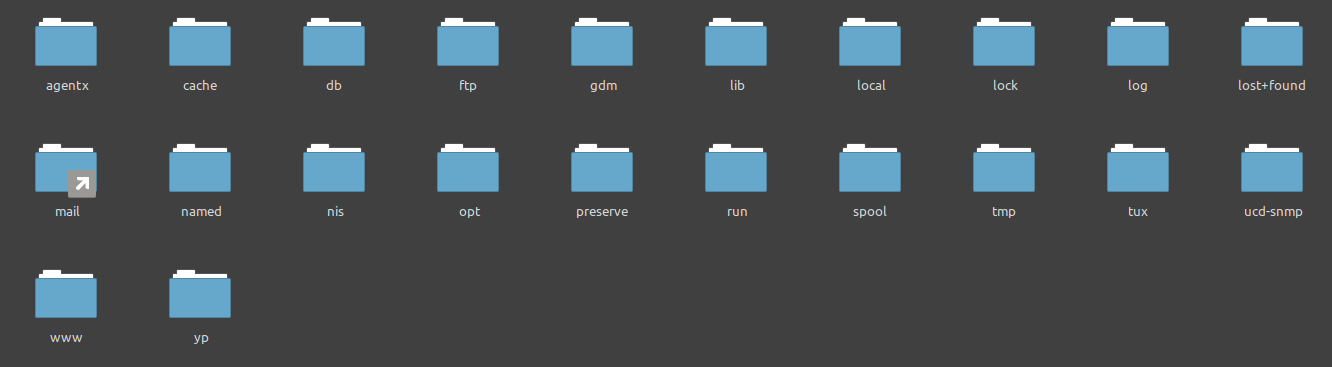
\includegraphics[width=0.5\linewidth]{givenFiles_var.png}
	\caption{We are given the 'var' folder from a compromised Linux host}
	\label{fig:givenFiles}
\end{figure}

The 'tmp' folder is empty so focusing on the log folder going forwards.


\printbibliography % Output the bibliography  

%----------------------------------------------------------------------------------------



%----------------------------------------------------------------------------------------
%	 Appendices
%----------------------------------------------------------------------------------------
%
%\appendix


%\clearpage
%\chapter{Appendices}
%\begin{appendices}

%\end{appendices}
\end{document}
